% Provenance (never printed): see sources/outline_sources.md (Year 2: the long-term carbon cycle
% and the silicate-weathering thermostat; Palaeozoic glaciations; the Cretaceous greenhouse; the
% PETM; Cenozoic cooling). Reservoirs from IPCC AR6 WG1 Figure 5.12; long-term fluxes after Derry
% (2024); weathering laws after Colbourn and others (2013); Phanerozoic CO2 after Foster and
% others (2017); Phanerozoic temperatures after Judd and others (2024); Cenozoic isotopes from
% CENOGRID (Westerhold 2020); the Eocene--Oligocene transition after Hutchinson and others (2021);
% the PETM after AR6 WG1 chapters 2 and 5. The thermostat model, its curves and every number of
% the exercises and problem from figdata/bachelor-2/deeptime.py and the Book 4 second-writer
% scratch calculator calc/ch26.py.
\chapter{Climate over Geological Time}\label{ch:b2:deep-time-climate}

Fifty million years ago no ice sheet stood anywhere on the Earth. The air held more than a
thousand parts per million of carbon dioxide, the poles had warmed far more than the equator, and
forests of a nearly tropical kind grew at \ang{70}~S, through the months of polar night. Thirty-four
million years ago ice spread over Antarctica, and it has never left. Over the hundreds of millions
of years recorded in the rocks, the Earth has swung between such worlds, with ice and without; yet
it has never boiled its oceans away nor frozen for good since the snowballs of
\cref{ch:b2:precambrian-earth}. This chapter follows the carbon that sets these climates, the slow
cycle that moves it between the air and the rocks, and the thermostat that keeps the planet
habitable.
% ledger: ipcc:ref-periods, ar6ch2:cenozoic, hutchinson21:eot

\begin{recall}
\textbf{From the school volumes}: the greenhouse effect and radiative forcing; the forcing of
carbon dioxide grows with the logarithm of its concentration, \qty{3.93}{W.m^{-2}} for a doubling;
equilibrium climate sensitivity, best estimate \qty{3}{\celsius}; outgassing; the glacial cycles
and the Last Glacial Maximum. \textbf{From the Year 1 volume}: chemical weathering and the
hydrolysis of silicates; clay minerals; carbonate oozes, the lysocline and the carbonate
compensation depth. \textbf{From earlier chapters}: the faint young Sun and \omterm{def:b2:precambrian-earth:snowball}{snowball Earth}
(\cref{ch:b2:precambrian-earth}); \omterm{def:b2:phanerozoic-earth:palaeogeography}{palaeogeography} and \omterm{def:b2:phanerozoic-earth:oae}{oceanic anoxic events}
(\cref{ch:b2:phanerozoic-earth}); climate proxies, $\delta^{18}$O and the \omterm{def:b2:climate-proxies:ice-volume}{ice-volume effect}
(\cref{ch:b2:climate-proxies}); orbital forcing (\cref{ch:b2:orbital-forcing}). The carbon cycle,
its reservoirs and the residence time belong to the biology books, the Arrhenius law to the
chemistry books.
\end{recall}
% ledger: ipcc:erf-2xco2, ipcc:log-co2, ipcc:ecs

\section{The long-term carbon cycle}\label{sec:b2:deep-time-climate:cycle}

\subsection*{Reservoirs and fluxes}

\begin{definition}[Long-term carbon cycle; carbonate--silicate cycle]\label{def:b2:deep-time-climate:carbon-cycle}
The \emph{long-term carbon cycle}\index{long-term carbon cycle} is the exchange of carbon between
the surface reservoirs (atmosphere, ocean, biosphere and soils) and the solid Earth: volcanic and
metamorphic degassing, the weathering of rocks, and the burial of carbonate and organic carbon in
sediments that later become rock or are subducted. Its fluxes are small against the surface
reservoirs and act over $10^5$ to $10^8$ years. The \emph{carbonate--silicate
cycle}\index{carbonate--silicate cycle} is its inorganic part: carbon dioxide leaves the mantle
and the crust at volcanoes, is consumed by the weathering of silicate rocks, is deposited on the
sea floor as carbonate, and returns to the surface when that carbonate is metamorphosed or
subducted and degassed.
\end{definition}
% ledger: derry24:fluxes, derry24:subduction, colbourn13:timescale

The biology books follow carbon through photosynthesis, respiration and the ocean over years to
centuries. On the time scale of climate history the picture widens to include the rocks. Before
the industrial era the atmosphere held \qty{591}{PgC} (petagrams, or billions of tonnes, of carbon);
the ocean held \num{38700}, nearly all of it as dissolved inorganic carbon in the intermediate and
deep water (\num{37100}); vegetation, soils and permafrost held \num{3350} between them. The
active surface reservoirs together hold about \num{3.5e6} teramoles of carbon, some
\qty{42000}{PgC}. The sedimentary rocks hold carbon too, as limestone and as organic matter
scattered through shales, and they exchange it with the surface only slowly.
% ledger: ar6ch5:fig512, derry24:residence

A modern estimate of the inputs and outputs, in teramoles of carbon a year ($\qty{1}{Tmol}$ of
carbon is \qty{0.012}{PgC}), runs as follows. Into the ocean and atmosphere: volcanic degassing at
mid-ocean ridges (1.3), ocean islands (1.3), arcs (4.5) and continental rifts (4.2), about 11 in
all; metamorphic degassing, 2 to 4; the weathering of old carbonate, 12.3, and the oxidation of
old organic carbon exposed by erosion, 8.1, with 2.0 from geological methane: \num{36.7} in all.
Out of them: carbonate sedimentation, about 26, and the burial of organic carbon, about 16. The two
sides balance within their uncertainties. Degassing from the Earth's interior supplies little more than a
third of the input (\cref{exo:b2:deep-time-climate:2}); the rest is old sedimentary carbon on its
way round again. Other estimates of the volcanic flux are lower, \qty{0.1}{PgC} a year
(about 8 Tmol) in the global carbon budget of the IPCC, or \qty{0.26}{Gt} of carbon dioxide (about 6
Tmol of carbon) in a survey of the US Geological Survey: the volcanic input is known to within a
factor of two.
% ledger: derry24:fluxes, ar6ch5:fig512, usgs:volcanic-co2

\begin{omfigure}
\centering
\begin{tikzpicture}[font=\scriptsize, >={Stealth[length=2mm]},
  box/.style={draw, thick, rounded corners=2pt, align=center, inner sep=4pt},
  up/.style={->, very thick, omThm}, down/.style={<-, very thick, omDef},
  lab/.style={midway, above, sloped, font=\scriptsize}]
% reservoirs: ar6ch5:fig512; active reservoirs derry24:residence; fluxes derry24:fluxes, derry24:subduction
\draw[thick, rounded corners=2pt, fill=blue!6] (-6.3,0) rectangle (6.0,2.6);
\node[anchor=north west, font=\small\bfseries] at (-6.2,2.55) {surface reservoirs, about \qty{42000}{PgC}};
\node[box, fill=white] (atm) at (-4.6,1.45) {atmosphere\\\qty{591}{PgC}};
\node[box, fill=white] (oc) at (0.6,1.45) {ocean\\\qty{38700}{PgC}};
\node[box, fill=white] (land) at (4.3,1.45) {vegetation, soils,\\permafrost \qty{3350}{PgC}};
\draw[->, very thick, omProp] (atm.east) -- (oc.west);
\node[align=center, text=omProp] at (-2.0,0.6) {silicate weathering 11--12, as bicarbonate};
\draw[<->, thick, black!50] (oc.east) -- (land.west);
% sedimentary rocks and mantle
\node[box, fill=brown!12, minimum width=5.7cm, minimum height=1.1cm] (rock) at (-3.35,-4.55) {sedimentary rocks:\\carbonate and organic carbon};
\node[box, fill=orange!15, minimum width=3.0cm, minimum height=1.1cm] (mantle) at (4.3,-4.55) {mantle};
% inputs (red, up) and outputs (blue, drawn upwards with the tip at the start)
\draw[up] (-5.7,-4.0) -- node[lab] {carbonate weathering 12.3} (-5.7,0);
\draw[up] (-4.8,-4.0) -- node[lab] {old organic C oxidised 8.1} (-4.8,0);
\draw[up] (-3.9,-4.0) -- node[lab] {geological methane 2.0} (-3.9,0);
\draw[up] (-3.0,-4.0) -- node[lab] {metamorphic degassing 2--4} (-3.0,0);
\draw[down] (-1.9,-4.0) -- node[lab] {carbonate sedimentation 26} (-1.9,0);
\draw[down] (-1.0,-4.0) -- node[lab] {organic carbon burial 16} (-1.0,0);
\draw[up] (4.3,-4.0) -- node[lab] {volcanoes, rifts 11.3} (4.3,0);
\draw[->, very thick, black!70] (rock.east) -- node[above] {subduction 4--6} (mantle.west);
\end{tikzpicture}
\par\smallskip{\small The \omterm{def:b2:deep-time-climate:carbon-cycle}{long-term carbon cycle}, with pre-industrial reservoirs from the IPCC's
global carbon budget and present fluxes from a 2024 synthesis, in teramoles of carbon a year
(\qty{1}{Tmol.yr^{-1}} = \qty{0.012}{PgC.yr^{-1}}). Red: inputs to the surface reservoirs; blue:
outputs. Silicate weathering does not leave the surface: it moves carbon from the air into the
ocean as bicarbonate, which then leaves as carbonate sediment.}
\end{omfigure}

Divided by the flux through them, the \qty{3.5e6}{Tmol} of the surface reservoirs give a
residence time of carbon of 8 to \num{9e4} years. Carbon that enters the ocean and air is buried
again within some hundred thousand years, a blink on the scale of this chapter: the surface
reservoirs follow the slow inputs and outputs closely, and any lasting imbalance between them
changes the carbon dioxide of the air.
% ledger: derry24:residence

\subsection*{Carbonate and silicate weathering}

Rain dissolves carbon dioxide and attacks rocks, as the Year 1 volume described. Two kinds of rock
behave very differently. Weathering a limestone takes one carbon dioxide from the air and one
carbon from the rock into the water; when a marine organism builds its shell from the products,
one carbon goes back to the air:
\[
  \ce{CaCO3 + CO2 + H2O -> Ca^{2+} + 2 HCO3^-} , \qquad
  \ce{Ca^{2+} + 2 HCO3^- -> CaCO3 + CO2 + H2O} .
\]
The round trip is null for the air. Weathering a silicate, written here with wollastonite as a
stand-in for the calcium silicates of granite and basalt, also takes carbon dioxide, but brings
none from the rock:
\[
  \ce{CaSiO3 + 2 CO2 + H2O -> Ca^{2+} + 2 HCO3^- + SiO2} ,
\]
and the carbonate built from it sends back only one of the two:
\[
  \ce{CaSiO3 + CO2 -> CaCO3 + SiO2} \quad\text{(net)} .
\]
Each mole of calcium or magnesium silicate weathered on land thus locks one mole of carbon dioxide
into carbonate rock. This is why carbonate sedimentation, about 26, exceeds carbonate weathering,
12.3, by roughly the 11 to 12 teramoles a year that silicate weathering consumes; and it is the
silicate weathering, not the carbonate, that balances the volcanoes over millions of years.
% ledger: colbourn13:timescale, derry24:fluxes

\section{The silicate-weathering thermostat}\label{sec:b2:deep-time-climate:thermostat}

\subsection*{A negative feedback}

Silicate weathering is a chemical reaction, and like most it is faster when it is warm. Warmth
also brings more rain and more run-off, which carry the products away and bring fresh water to the
rock. The rate therefore rises with temperature; and temperature rises with the carbon dioxide of
the air. A planet that gains carbon dioxide warms, weathers faster and loses it again.

\begin{definition}[Silicate-weathering thermostat]\label{def:b2:deep-time-climate:thermostat}
The \emph{silicate-weathering thermostat}\index{silicate-weathering thermostat} is the negative
feedback between climate and the \omterm{def:b2:deep-time-climate:carbon-cycle}{long-term carbon cycle}: the weathering of silicate rocks, which
removes carbon dioxide from the atmosphere into carbonate rock, increases with temperature and
run-off, so that a rise of atmospheric carbon dioxide raises the rate of its own removal and a
fall lowers it. Over $10^5$ to $10^6$ years it brings the removal back into balance with the
degassing.
\end{definition}
% ledger: colbourn13:timescale, colbourn13:weathering, hutchinson21:gateways

The temperature dependence is that of the Arrhenius law of the chemistry books. With an activation
energy $E_{\text a}$ for the dissolution of calcium and magnesium silicates, the weathering flux at
a temperature $T$ near a reference $T_0$ is
\[
  W = W_0 \exp\Bigl[-\frac{E_{\text a}}{R}\Bigl(\frac1T - \frac1{T_0}\Bigr)\Bigr]
  \approx W_0\, e^{k_T (T - T_0)}, \qquad k_T = \frac{E_{\text a}}{R T_0^2},
\]
since $1/T - 1/T_0 \approx -(T - T_0)/T_0^2$. Laboratory dissolution gives $E_{\text a} =
\qty{63}{kJ.mol^{-1}}$, and with $T_0 = \qty{288}{K}$, $k_T = \qty{0.09}{K^{-1}}$: the flux grows
by about \qty{9}{\percent} for each degree; within ten degrees of $T_0$ the approximation departs
from the exact law by less than \qty{3}{\percent} (\cref{exo:b2:deep-time-climate:6}). A field estimate is
$74 \pm \qty{29}{kJ.mol^{-1}}$, so the sensitivity is uncertain by a factor of about two. Run-off
adds to it: with a flux proportional to $(R/R_0)^{0.65}$ and a run-off that rises by
\qty{4.5}{\percent} per degree, the combined sensitivity becomes $k = 0.09 + 0.65\times0.045 =
\qty{0.119}{K^{-1}}$.
% ledger: colbourn13:weathering
% values: k_run 0.11925 (deeptime.py)

\subsection*{A one-box model}

To see how fast the thermostat works, follow the excess carbon $M$ that the ocean and atmosphere
hold above a steady state. Within a few thousand years of a disturbance the ocean and the sea-floor
carbonates have taken most of an excess out of the air; for a release of \qty{4000}{PgC}, about
\qty{8}{\percent} stays in the air until silicate weathering removes it. Write $f$ for that
fraction and $A_0 = \qty{591}{PgC}$ for the air's pre-industrial carbon, so that the carbon dioxide
of the air is $C = C_0(1 + fM/A_0)$. The warming follows the logarithmic law with the climate
sensitivity $S$, $\Delta T = S\log_2(C/C_0)$, and the weathering follows the exponential law above.
% ledger: colbourn13:timescale, ar6ch5:fig512, ipcc:ecs, ipcc:log-co2

\begin{proposition}[The thermostat's steady state and time constant]\label{prop:b2:deep-time-climate:thermostat}
Let the excess carbon $M$ of the ocean--atmosphere change as
\[
  \frac{\mathrm dM}{\mathrm dt} = V - W_0\,e^{k\,\Delta T(M)}, \qquad
  \Delta T(M) = S\log_2\Bigl(1 + \frac{fM}{A_0}\Bigr),
\]
where $V$ is the degassing and $W_0$ the weathering at $M = 0$.
\begin{enumerate}
  \item The steady state has $\Delta T^* = \ln(V/W_0)/k$, whatever $S$ and $f$.
  \item If $V = W_0$, a small excess decays as $M(t) = M(0)\,e^{-t/\tau}$ with
        \[
          \tau = \frac{A_0 \ln 2}{f\,k\,S\,W_0} .
        \]
\end{enumerate}
\end{proposition}

\begin{proof}
(1) At a steady state $\mathrm dM/\mathrm dt = 0$, so $W_0e^{k\Delta T^*} = V$ and $\Delta T^* =
\ln(V/W_0)/k$; neither $S$ nor $f$ enters. (2) Near $M = 0$, $\log_2(1 + x) \approx x/\ln 2$, so
$\Delta T \approx SfM/(A_0\ln 2)$ and $e^{k\Delta T} \approx 1 + kSfM/(A_0\ln2)$. With $V = W_0$ the
equation becomes $\mathrm dM/\mathrm dt = -W_0kSfM/(A_0\ln 2) = -M/\tau$, whose solution is the
exponential.
\end{proof}

The first result is the heart of the thermostat. It fixes a temperature, not a concentration: if
the volcanoes degas \qty{20}{\percent} more, the Earth settles $\ln 1.2/0.09 = \qty{2.0}{\celsius}$
warmer, whatever its climate sensitivity, and the carbon dioxide adjusts to whatever gives that
warming, here \qty{60}{\percent} more. A weak weathering response, a small $k$, makes a poor
thermostat; a strong one holds the temperature nearly fixed.
% values: dT_step 2.026, C_step_ratio 1.597 (deeptime.py)

\begin{example}[The thermostat's time constant]\label{ex:b2:deep-time-climate:tau}
Silicate weathering consumes 11 to \qty{12}{Tmol} of carbon a year; take $W_0 = 11.5\times0.012011
= \qty{0.138}{PgC.yr^{-1}}$. With $A_0 = \qty{591}{PgC}$, $f = 0.08$, $k = \qty{0.09}{K^{-1}}$ and
$S = \qty{3}{K}$,
\[
  \tau = \frac{591\times0.693}{0.08\times0.09\times3\times0.138} = \qty{1.37e5}{yr} ,
\]
about 140 thousand years. With the run-off factor, $k = 0.119$, it shortens to
\qty{104}{kyr}.
\end{example}
% ledger: derry24:fluxes, ar6ch5:fig512, colbourn13:timescale, colbourn13:weathering, ipcc:ecs
% values: tau_kT_kyr 137.3, tau_run_kyr 103.6 (deeptime.py)

The model is crude: the fraction $f$ is not a constant, the ocean's chemistry is reduced to one
number and the weathering to one global law. Models with an explicit ocean and sediment give
e-folding times from about \qty{200}{kyr} to a million years. The thermostat is therefore a
regulator of the very long term: it does nothing to the climate of the next few thousand years, and
it holds the Earth's temperature within bounds over hundreds of millions.
% ledger: colbourn13:timescale

\begin{omfigure}
\centering
\begin{tikzpicture}
\begin{groupplot}[group style={group size=2 by 1, horizontal sep=1.6cm},
  omrecord, width=0.47\linewidth, height=5.4cm, xmin=0, xmax=1000,
  xlabel={time (\unit{kyr})}, xtick pos=bottom, ytick pos=left,
  tick label style={font=\scriptsize}, label style={font=\small},
  legend style={draw=none, fill=white, font=\scriptsize}]
\nextgroupplot[ymin=0, ymax=5200, ylabel={excess carbon (\unit{PgC})},
  y tick label style={/pgf/number format/1000 sep={\,}},
  legend style={at={(0.97,0.97)}, anchor=north east}]
% computed in figdata/bachelor-2/deeptime.py part pulse; ledger: colbourn13:timescale, colbourn13:weathering, derry24:fluxes, ar6ch5:fig512, ipcc:ecs
\addplot[omThm, line width=1.2pt] table[x=t_kyr, y=M_nl] {figdata/out/bachelor-2-deeptime-pulse.dat};
\addlegendentry{model}
\addplot[black, densely dashed, line width=1.0pt] table[x=t_kyr, y=M_lin] {figdata/out/bachelor-2-deeptime-pulse.dat};
\addlegendentry{linearised}
\draw[densely dotted] (axis cs:137.3,0) -- (axis cs:137.3,1839);
\node[anchor=west, font=\scriptsize] at (axis cs:145,1400) {$\tau$};
\nextgroupplot[ymin=0, ymax=2.4, ylabel={warming (\unit{\celsius})},
  legend style={at={(0.97,0.03)}, anchor=south east}]
% computed in figdata/bachelor-2/deeptime.py part step
\addplot[omThm, line width=1.2pt] table[x=t_kyr, y=dT_nl] {figdata/out/bachelor-2-deeptime-step.dat};
\addlegendentry{model}
\addplot[black, densely dashed, line width=1.0pt] table[x=t_kyr, y=dT_lin] {figdata/out/bachelor-2-deeptime-step.dat};
\addlegendentry{linearised}
\draw[densely dotted] (axis cs:0,2.026) -- (axis cs:1000,2.026);
\node[anchor=south east, font=\scriptsize] at (axis cs:1000,2.03) {$\ln 1.2/k$};
\end{groupplot}
\end{tikzpicture}
\par\smallskip{\small The one-box thermostat with $k = \qty{0.09}{K^{-1}}$ and $S = \qty{3}{K}$.
Left: a release of \qty{5000}{PgC} at time zero, counted after the ocean and the carbonates have
taken their share; it decays with the e-folding time $\tau$, a little more slowly than the
linearised law at first. Right: the degassing raised by \qty{20}{\percent} at time zero; the Earth
warms towards the steady \qty{2.0}{\celsius} of \cref{prop:b2:deep-time-climate:thermostat}.}
\end{omfigure}
% values: t90_lin_kyr 316.2, t90_nl_kyr 339.9, tau_step_kyr 182.7 (deeptime.py)

The thermostat also explains the faint young Sun of \cref{ch:b2:precambrian-earth}. The Sun brightens
by a few per cent every few hundred million years, and an Earth with fixed air would warm with it;
but warmer means faster weathering, which draws the carbon dioxide down until the temperature
returns close to where the degassing puts it. The rocks of the last 420 million years show exactly
this, as the next section reads.

\section{Greenhouse and icehouse worlds}\label{sec:b2:deep-time-climate:states}

\begin{definition}[Greenhouse and icehouse climate states]\label{def:b2:deep-time-climate:states}
A \emph{greenhouse climate state}\index{greenhouse climate state} is a long interval, millions to
tens of millions of years, without large continental ice sheets, with high atmospheric carbon
dioxide and a small temperature difference between the equator and the poles. An \emph{icehouse
climate state}\index{icehouse climate state} is a long interval with continental ice sheets at one
or both poles, lower carbon dioxide and a steep equator-to-pole gradient. The Earth has been in an
icehouse state since about \qty{34}{Ma}.
\end{definition}
% ledger: judd24:phanda, hutchinson21:eot

\subsection*{Carbon dioxide over 420 million years}

Carbon dioxide before the ice cores is read from proxies: the boron isotopes and organic molecules
of marine plankton, the pores of fossil leaves, the carbonate nodules of ancient soils. A 2017
compilation of them back to \qty{420}{Ma}, smoothed, is shown below with the glaciations. Its
long-term trend is a decline of about \qty{3.4}{ppm} per million years, and values close to the
pre-industrial level appear twice before our own time: in the Carboniferous and Permian, and
briefly in the late Cretaceous.
% ledger: foster17:co2, data:b4-foster2017, ar6ch2:deep-co2

\begin{omfigure}
\centering
\begin{tikzpicture}
\begin{axis}[omrecord, omage, width=0.92\linewidth, height=6.4cm, xmin=0, xmax=450, ymode=log,
  ymin=80, ymax=8000, xlabel={age (\unit{Ma})}, ylabel={carbon dioxide (\unit{ppm})},
  xtick={0,50,...,400}, ytick={100,200,500,1000,2000,5000}, yticklabels={100,200,500,1000,2000,5000},
  xtick pos=bottom, ytick pos=left, clip=false,
  tick label style={font=\scriptsize}, label style={font=\small}]
% computed in figdata/bachelor-2/deeptime.py part co2; ledger: data:b4-foster2017, foster17:co2, judd24:phanda, hutchinson21:eot, ar6ch5:cenozoic-co2, ics:base.Ordovician, ics:base.Silurian, ics:base.Devonian, ics:base.Carboniferous, ics:base.Permian, ics:base.Triassic, ics:base.Jurassic, ics:base.Cretaceous, ics:base.Paleogene, ics:base.Neogene, ics:colour.Ordovician, ics:colour.Silurian, ics:colour.Devonian, ics:colour.Carboniferous, ics:colour.Permian, ics:colour.Triassic, ics:colour.Jurassic, ics:colour.Cretaceous, ics:colour.Paleogene, ics:colour.Neogene
\fill[blue!12] (axis cs:445.21,80) rectangle (axis cs:443.07,8000);
\fill[blue!12] (axis cs:371.1,80) rectangle (axis cs:298.89,8000);
\fill[blue!12] (axis cs:34,80) rectangle (axis cs:0,8000);
\addplot[name path=hi, draw=none, forget plot] table[x=age, y=hi68] {figdata/out/bachelor-2-deeptime-co2.dat};
\addplot[name path=lo, draw=none, forget plot] table[x=age, y=lo68] {figdata/out/bachelor-2-deeptime-co2.dat};
\addplot[omDef!25, forget plot] fill between[of=hi and lo];
\addplot[omDef, line width=1.2pt] table[x=age, y=co2] {figdata/out/bachelor-2-deeptime-co2.dat};
\addplot[black!60, densely dashed] coordinates {(0,278) (450,278)};
\node[anchor=south west, font=\scriptsize, text=black!70] at (axis cs:440,280) {pre-industrial};
\node[anchor=north west, font=\scriptsize, text=blue!60!black, align=left] at (axis cs:442,7600) {Late\\Ordovician};
\node[anchor=north, font=\scriptsize, text=blue!60!black, align=center] at (axis cs:335,7600) {late Palaeozoic\\ice age};
\node[anchor=north, font=\scriptsize, text=blue!60!black, align=center] at (axis cs:17,7600) {Cenozoic\\ice};
\foreach \a/\b/\c in {450/443.1/icsOrdovician, 443.1/419.62/icsSilurian, 419.62/358.86/icsDevonian, 358.86/298.9/icsCarboniferous,
  298.9/251.902/icsPermian, 251.902/201.4/icsTriassic, 201.4/143.1/icsJurassic,
  143.1/66/icsCretaceous, 66/23.04/icsPaleogene, 23.04/0/icsNeogene} {
  \edef\tmp{\noexpand\fill[\c] (axis cs:\a,80) rectangle (axis cs:\b,95);}\tmp}
\node[font=\tiny] at (axis cs:431.4,87) {S};
\node[font=\tiny] at (axis cs:389.2,87) {D};
\node[font=\tiny] at (axis cs:328.9,87) {C};
\node[font=\tiny] at (axis cs:275.4,87) {P};
\node[font=\tiny] at (axis cs:226.7,87) {T};
\node[font=\tiny] at (axis cs:172.3,87) {J};
\node[font=\tiny] at (axis cs:104.6,87) {K};
\node[font=\tiny] at (axis cs:44.5,87) {Pg};
\end{axis}
\end{tikzpicture}
\par\smallskip{\small Atmospheric carbon dioxide over the last 420 million years: the smoothed fit
(line) to a compilation of proxy estimates, with its \qty{68}{\percent} band, on a logarithmic
scale. Blue bands: the Hirnantian glaciation of the Late Ordovician; the late Palaeozoic ice age,
from its first glacial deposits in the latest Devonian to its greatest ice extent at the end of the
Carboniferous; the Cenozoic ice since \qty{34}{Ma}. The bar at the foot shows the periods.}
\end{omfigure}

Over the same 420 million years the Sun brightened by about \qty{4}{\percent}, some
\qty{50}{W.m^{-2}} at the Earth's distance and \qty{9}{W.m^{-2}} of forcing once spread over the
sphere and corrected for the albedo. The fall of carbon dioxide from about \qty{1400}{ppm} to the
pre-industrial value almost exactly cancels it (\cref{exo:b2:deep-time-climate:7}): in terms of
forcing the Earth has stayed within a few watts per square metre of today for 420 million years,
and its icehouse states came when the combined forcing of carbon dioxide and Sun fell below about 1
to \qty{2}{W.m^{-2}}. The authors of the compilation attribute the compensation to the silicate
weathering feedback and the spread of land plants, whose roots and soils speed weathering.
% ledger: foster17:co2, data:b4-foster2017, ipcc:erf-2xco2

\subsection*{Palaeozoic ice ages}

A reconstruction of global mean surface temperature published in 2024, which combines proxy data
with climate models, puts the Phanerozoic range between \qty{11}{\celsius}, in the glacial times of
the late Pleistocene, 129 to 11.7 thousand years ago, and \qty{36}{\celsius}, in the Turonian, 94 to \qty{89}{Ma} ago.
Its warm and cold intervals follow the glaciations recorded by tillites and striated pavements.
% ledger: judd24:phanda

The Late Ordovician glaciation, in the Hirnantian stage (445.2 to \qty{443.1}{Ma}), spread ice sheets
over Gondwana, much of which lay near the South Pole (\cref{ch:b2:phanerozoic-earth}), and
coincided with one of the five great extinctions. Its global mean temperature, about
\qty{21}{\celsius} in the reconstruction, is warmer than that of later glaciations: the vast
\omterm{def:b2:wilson-cycle:supercontinent}{supercontinent} made its interior cold enough for ice sheets anyway. The late Palaeozoic ice age is
the longest of the Phanerozoic: its first glacial deposits are latest Devonian, its coldest global
temperatures in the Serpukhovian, about 330 to \qty{323}{Ma}, and its greatest extent
of ice towards the end of the Carboniferous, 307 to \qty{299}{Ma}. It coincides with the low carbon
dioxide of the Carboniferous and Permian, which the compilation's authors link to a weaker volcanic
flux or stronger weathering while Pangaea was assembled and its mountains stood high.
% ledger: judd24:phanda, ar6ch2:deep-co2, foster17:co2, ics:base.Silurian

\subsection*{The Cretaceous greenhouse}

The warmest time of the reconstruction is the middle Cretaceous, the time of the high seas and the
\omterm{def:b2:phanerozoic-earth:oae}{oceanic anoxic events} of \cref{ch:b2:phanerozoic-earth}. The carbon dioxide estimates for
it are puzzling: the compilation above gives some 450 to \qty{860}{ppm} between 100 and
\qty{90}{Ma}, and the 2024 reconstruction finds a median of about \qty{775}{ppm} for its hottest
intervals, lower than its temperatures suggest. Whether carbon dioxide and temperature truly parted
company then, or the proxies misread the Cretaceous air, is open; the authors call it the ``Mesozoic
conundrum''.
% ledger: judd24:phanda, data:b4-foster2017

\section{The Cenozoic: from hothouse to icehouse}\label{sec:b2:deep-time-climate:cenozoic}

The best record of the last 66 million years is in the shells of benthic foraminifera, cored from
the deep-sea floor. Their $\delta^{18}$O rises when the deep water cools and when ice sheets store
the light isotope on land (\cref{ch:b2:climate-proxies}). The figure below shows the reference
record built in 2020 from deep-sea drill cores, averaged over \qty{100}{kyr}.
% ledger: data:b4-cenogrid, ar6ch2:cenozoic

\begin{omfigure}
\centering
\begin{tikzpicture}
\begin{axis}[omrecord, omage, width=0.92\linewidth, height=6.4cm, xmin=0, xmax=67,
  ymin=-1.2, ymax=5.6, y dir=reverse, xlabel={age (\unit{Ma})},
  ylabel={benthic $\delta^{18}$O (\unit{\permil})}, xtick={0,10,...,60},
  xtick pos=bottom, ytick pos=left, clip=false,
  tick label style={font=\scriptsize}, label style={font=\small}]
% computed in figdata/bachelor-2/deeptime.py part ceno; ledger: data:b4-cenogrid, ar6ch2:cenozoic, ar6ch5:cenozoic-co2, hutchinson21:eot, ipcc:ref-periods, ar6ch5:petm
\fill[omThm!15] (axis cs:53,-1.2) rectangle (axis cs:49,5.6);
\fill[omThm!15] (axis cs:16.9,-1.2) rectangle (axis cs:14.7,5.6);
\addplot[black!45, line width=0.4pt] table[x=age, y=d18O] {figdata/out/bachelor-2-deeptime-ceno.dat};
\addplot[omDef, line width=1.3pt] table[x=age, y=d18O_lt] {figdata/out/bachelor-2-deeptime-ceno.dat};
\draw[omThm, thick, ->] (axis cs:55.85,-0.7) -- (axis cs:55.85,-1.15);
\node[anchor=south, font=\scriptsize, text=omThm] at (axis cs:55.85,-1.15) {PETM};
\node[anchor=north, font=\scriptsize, text=omThm] at (axis cs:51,4.6) {EECO};
\node[anchor=north, font=\scriptsize, text=omThm] at (axis cs:15.8,0.6) {MCO};
\draw[blue!60!black, densely dashed] (axis cs:33.9,-1.2) -- (axis cs:33.9,5.6);
\node[anchor=south west, font=\scriptsize, text=blue!60!black, align=left] at (axis cs:33.6,4.4)
  {Antarctic ice\\from \qty{34}{Ma}};
\draw[blue!60!black, densely dashed] (axis cs:2.7,-1.2) -- (axis cs:2.7,5.6);
\node[anchor=north west, font=\scriptsize, text=blue!60!black, align=left] at (axis cs:2.5,-0.9)
  {northern\\ice sheets};
\node[anchor=south west, font=\scriptsize, align=left] at (axis cs:66.3,5.45) {colder, more ice $\downarrow$};
\end{axis}
\end{tikzpicture}
\par\smallskip{\small Deep-sea benthic foraminiferal $\delta^{18}$O over the Cenozoic, from the
CENOGRID reference splice: \qty{100}{kyr} means (grey) and the dataset's long-term smoothing
(blue). The axis is reversed, so that colder and icier is down. Shaded: the Early Eocene Climatic
Optimum (EECO) and the Miocene Climatic Optimum (MCO); dashed: the start of the Antarctic ice
sheet and the major advances of the northern ice sheets.}
\end{omfigure}

Read from right to left, the record tells four chapters. The early Cenozoic warmed, through the
\omterm{def:b2:deep-time-climate:petm}{Palaeocene--Eocene Thermal Maximum}, to the Early Eocene Climatic Optimum, 53 to \qty{49}{Ma}, when
global temperature stood 10 to \qty{18}{\celsius} above that of 1850--1900 (\emph{medium
confidence}, in the language of the IPCC) and carbon dioxide between 1150 and \qty{2500}{ppm}.
A long cooling followed, punctuated at the Eocene--Oligocene transition, about \qty{34}{Ma}, by a
jump of about \qty{1.5}{\permil} in $\delta^{18}$O: the first large ice sheet on Antarctica, with a
deep-ocean cooling of the order of \qty{2}{\celsius}. The Miocene Climatic Optimum, 16.9 to
\qty{14.7}{Ma}, brought warmth back, 4 to \qty{10}{\celsius} above 1850--1900 with 400 to
\qty{600}{ppm}. After the mid-Pliocene, the last time carbon dioxide stood near today's 360 to
\qty{420}{ppm}, it fell by some \qty{30}{ppm} per million years, and from \qty{2.7}{Ma} ice sheets
grew durably in the northern hemisphere: the glacial cycles of \cref{ch:b2:orbital-forcing} began.
% ledger: ipcc:mpwp-eeco, ar6ch2:deep-co2, ipcc:ref-periods, ar6ch2:mco, ar6ch2:mco-co2, hutchinson21:eot, ar6ch5:cenozoic-co2, ipcc:likelihood

Over the whole of the last 50 million years carbon dioxide fell at about \qty{16}{ppm} per million
years. The IPCC calls the cause uncertain, possibly an imbalance between volcanic degassing and the
two long-term sinks, organic carbon burial and silicate weathering. A threshold of 750 to
\qty{1000}{ppm} has been modelled for the growth of permanent ice sheets on Antarctica; the last time
carbon dioxide stood as high as \qty{1000}{ppm} was just before the transition.
% ledger: ar6ch5:cenozoic-co2, ar6ch2:deep-co2

\begin{dated}{2023}
In 2023 a consortium of researchers published a vetted compilation of all the Cenozoic carbon
dioxide estimates then published. In its reconstruction carbon dioxide peaked near \qty{1600}{ppm} around
\qty{51}{Ma}; the onset of the Antarctic ice sheet, near \qty{33.9}{Ma}, came at \qty{720}{ppm}; by
\qty{32}{Ma} it had fallen to \qty{550}{ppm}; the Middle Miocene, about \qty{16}{Ma}, was the last
time it stayed higher than today; and it fell below \qty{270}{ppm} at \qty{2.6}{Ma}, when the Earth
entered its present state of ice at both poles. Read against temperature, the curve gives an
\emph{Earth system sensitivity} --- the warming per doubling once ice sheets and vegetation have
responded --- of about \qty{8}{\celsius} through the cooling to \qty{34}{Ma}, or \qty{5}{\celsius}
with another temperature record: more than the \qty{3}{\celsius} of the fast feedbacks.
\end{dated}
% ledger: cenco2pip23:co2, ipcc:ecs

\subsection*{Tectonics and climate}

Why did carbon dioxide fall? Two families of explanation draw on plate tectonics, and the IPCC's
summary names both: the drift of the plates built mountains, drove erosion and volcanism and
reconfigured the ocean passages, and so moved carbon from the atmosphere into other reservoirs.
% ledger: ar6ch2:cenozoic

The first is weathering. Mountains weather faster than lowlands: steep slopes are scoured of their
soil, and fresh rock is exposed to rain. The uplift of the Himalaya and the Tibetan Plateau since
the India--Asia collision of \cref{ch:b2:himalaya-andes} has been proposed to have raised global
silicate weathering and drawn the carbon dioxide down. The thermostat makes this subtle: if the
Earth's ``weatherability'', the factor $W_0$, rises at a fixed degassing, the steady temperature
falls by $\ln(W_0'/W_0)/k$ (\cref{exo:b2:deep-time-climate:9}), but the thermostat still holds the
removal equal to the degassing. Uplift changes the climate at which the balance is struck, not the
balance itself. The hypothesis remains debated.
% ledger: hutchinson21:gateways, colbourn13:weathering

\begin{definition}[Ocean gateway]\label{def:b2:deep-time-climate:gateway}
An \emph{ocean gateway}\index{ocean gateway} is a strait or passage between two oceans whose opening,
closing or deepening by plate motion changes the exchange of water, heat and salt between them, and
so the ocean circulation.
\end{definition}

The second is the \omterm{def:b2:deep-time-climate:gateway}{ocean gateways}, above all the Drake Passage between South America and Antarctica
and the Tasman Gateway between Australia and Antarctica. Once both were deep, a current could flow
right round Antarctica. The Tasman Gateway deepened beyond about \qty{500}{m} at $33.5 \pm
\qty{1.5}{Ma}$, close to the transition; the Drake Passage opened earlier, perhaps by \qty{50}{Ma},
but shallow and narrow, and ridges may have blocked deep flow through it until about \qty{22}{Ma}. Models with
the geography of the Eocene find that opening the gateways changes the heat carried towards
Antarctica only modestly; the review of 2021 concludes that a fall of carbon dioxide, of perhaps
\qty{40}{\percent}, best explains the transition, with the gateways and the ice sheet itself in a
secondary role.
% ledger: hutchinson21:gateways, hutchinson21:eot

\section{Hyperthermals and the PETM}\label{sec:b2:deep-time-climate:petm}

The slow decline of carbon dioxide is interrupted by a few sudden spikes.

\begin{definition}[Hyperthermal event; Palaeocene--Eocene Thermal Maximum]\label{def:b2:deep-time-climate:petm}
A \emph{hyperthermal event}\index{hyperthermal event} is a geologically brief global warming, a few
thousand to a few hundred thousand years long, caused by a rapid release of carbon to the ocean and
atmosphere and recorded by a fall of the $\delta^{13}$C of marine and terrestrial carbon, a
dissolution of sea-floor carbonate and a fall of $\delta^{18}$O. The \emph{Palaeocene--Eocene
Thermal Maximum}\index{Palaeocene--Eocene Thermal Maximum} (PETM), 55.9 to \qty{55.7}{Ma}, is the
largest of the Cenozoic; its onset marks the base of the Eocene.
\end{definition}
% ledger: ar6ch5:petm, gssp:ypresian, ics4:eocene

\begin{omfigure}
\centering
\begin{tikzpicture}
\begin{groupplot}[group style={group size=1 by 2, vertical sep=0.25cm, x descriptions at=edge bottom},
  omrecord, omage, width=0.86\linewidth, height=4.1cm, xmin=55.5, xmax=56.3,
  xlabel={age (\unit{Ma})}, xtick={55.5,55.6,...,56.3},
  x tick label style={/pgf/number format/.cd, fixed, fixed zerofill, precision=1},
  xtick pos=bottom, ytick pos=left, tick label style={font=\scriptsize}, label style={font=\small}]
\nextgroupplot[ymin=-3, ymax=2, ylabel={$\delta^{13}$C (\unit{\permil})}]
% computed in figdata/bachelor-2/deeptime.py part petm; ledger: data:b4-cenogrid, ar6ch5:petm
\addplot[omDef, line width=0.9pt] table[x=age, y=d13C] {figdata/out/bachelor-2-deeptime-petm.dat};
\draw[densely dotted] (axis cs:56.3,1.32) -- (axis cs:55.5,1.32);
\node[anchor=south west, font=\scriptsize] at (axis cs:56.28,1.35) {before};
\draw[<->, omThm, thick] (axis cs:55.80,1.32) -- (axis cs:55.80,-2.41);
\node[anchor=west, font=\scriptsize, text=omThm] at (axis cs:55.795,-1.6) {\qty{3.7}{\permil}};
\nextgroupplot[ymin=-3, ymax=1.5, y dir=reverse, ylabel={$\delta^{18}$O (\unit{\permil})}]
\addplot[omThm, line width=0.9pt] table[x=age, y=d18O] {figdata/out/bachelor-2-deeptime-petm.dat};
\node[anchor=north east, font=\scriptsize, align=right] at (axis cs:55.52,-2.9) {warmer $\uparrow$};
\end{groupplot}
\end{tikzpicture}
\par\smallskip{\small The PETM in the CENOGRID splice, on its grid of \qty{5}{kyr}. Top: benthic
$\delta^{13}$C falls by about \qty{3.7}{\permil} from its mean before the event; bottom:
$\delta^{18}$O, axis reversed, falls as the deep sea warms. The straight stretch from 55.93 to
\qty{55.865}{Ma} is not a slow onset: no shell was measured there, and the splice joins the last
point before the event to the first one inside it. The recovery, from right to left, takes a
hundred thousand years.}
\end{omfigure}
% values: d13C pre 1.32, min -2.41 at 55.835; d18O pre 0.19, min -2.46 (data:b4-cenogrid)

The IPCC's assessment of the PETM runs as follows. Carbon dioxide rose from about 900 to more than
\qty{2000}{ppm}; the carbon was released in 3 to \qty{20}{kyr}, between about 3000 and more than
\qty{7000}{PgC} of it (\emph{low to medium confidence}), from methane hydrates, volcanoes, organic
carbon on land and at sea, or a combination. The Earth warmed by 4 to \qty{8}{\celsius} above
pre-industrial, about \qty{5}{\celsius} above the climate just before the event; the rise of carbon
dioxide inferred so far accounts for only about half of that warming. The surface ocean's pH fell
by 0.15 to 0.30; the carbonate saturation horizon rose within less than \qty{10}{kyr} and sea-floor
carbonate dissolved, then recovered gradually over some \qty{100}{kyr} (\emph{medium confidence}
that this was global). The light carbon of the release is why $\delta^{13}$C fell: the carbon
isotope record of such events belongs to the Year 3 volume.
% ledger: ar6ch5:petm, ar6ch5:petm-release, ipcc:mpwp-eeco, ar6ch2:deep-co2, ipcc:likelihood

\begin{omfigure}
\centering
\begin{tikzpicture}[x=0.052cm, y=1cm, font=\scriptsize]
% schematic; durations from ar6ch5:petm (onset 3-20 kyr, saturation horizon <10 kyr, recovery about 100 kyr; event 55.9-55.7 Ma)
\draw[->] (0,0) -- (215,0) node[anchor=west] {time (\unit{kyr})};
\foreach \t in {0,50,100,150,200} {\draw (\t,0) -- (\t,-0.1) node[anchor=north] {\t};}
\fill[omThm!70] (0,0.3) rectangle (20,0.8);
\fill[omThm!35] (20,0.3) rectangle (100,0.8);
\fill[omDef!30] (100,0.3) rectangle (200,0.8);
\node at (60,0.55) {warm body};
\node at (150,0.55) {recovery about \qty{100}{kyr}};
\draw[decorate, decoration={brace, amplitude=4pt}] (0,0.85) -- (20,0.85)
  node[midway, above=4pt] {onset, 3--20};
\node[anchor=west, align=left] at (0,1.75) {carbon released, \numrange{3000}{7000}~\unit{PgC}; warming
  4--\qty{8}{\celsius} above pre-industrial};
\end{tikzpicture}
\par\smallskip{\small The PETM as a sequence (schematic): a release of carbon over 3 to
\qty{20}{kyr}, a warm interval, and a recovery of the ocean's carbonate over about \qty{100}{kyr};
the whole event spans some \qty{200}{kyr}. The length of the warm body is drawn to fill the
interval, not measured.}
\end{omfigure}

How did the Earth recover? The thermostat is one candidate the IPCC names, with the regrowth of
organic carbon on land and at sea. The one-box model gives a hint of the answer. A release of
\qty{5000}{PgC} leaves \qty{400}{PgC} in the air once the ocean and the carbonates have acted, and
the thermostat removes \qty{90}{\percent} of the excess in $\tau\ln 10 \approx \qty{320}{kyr}$ for
$\tau = \qty{137}{kyr}$ --- longer than the recovery recorded at the PETM. Either the weathering
was more sensitive than the model's, as the run-off factor and the larger Earth system sensitivity
both suggest, or the regrowth of organic carbon did part of the work. The rates also differ from
today's: the PETM's carbon was released at 0.3 to \qty{1.5}{PgC} a year, and the carbon dioxide of
its air rose by 4 to \qty{42}{ppm} a century, at least four to five times slower than in 1995--2014.
% ledger: ar6ch5:petm, ar6ch5:petm-release, colbourn13:timescale, cenco2pip23:co2
% values: C_pulse0_ratio 1.677, t90_lin_kyr 316.2 (deeptime.py)

\begin{inthelab}[Reading a hyperthermal in a core]
In a deep-sea core that crosses the PETM, the carbonate content of the sediment drops abruptly
where the sea floor's carbonate dissolved, and returns gradually above. The scientists sample the
interval closely, pick the shells of one genus of benthic foraminifera under the binocular
microscope, and measure their $\delta^{13}$C and $\delta^{18}$O on a mass spectrometer. Records from
several sites are then spliced onto one time scale, tuned to the orbital cycles of
\cref{ch:b2:orbital-forcing}, which resolves the onset to a few thousand years.
\end{inthelab}
% ledger: ar6ch5:petm, data:b4-cenogrid

\begin{omfigure}
\centering
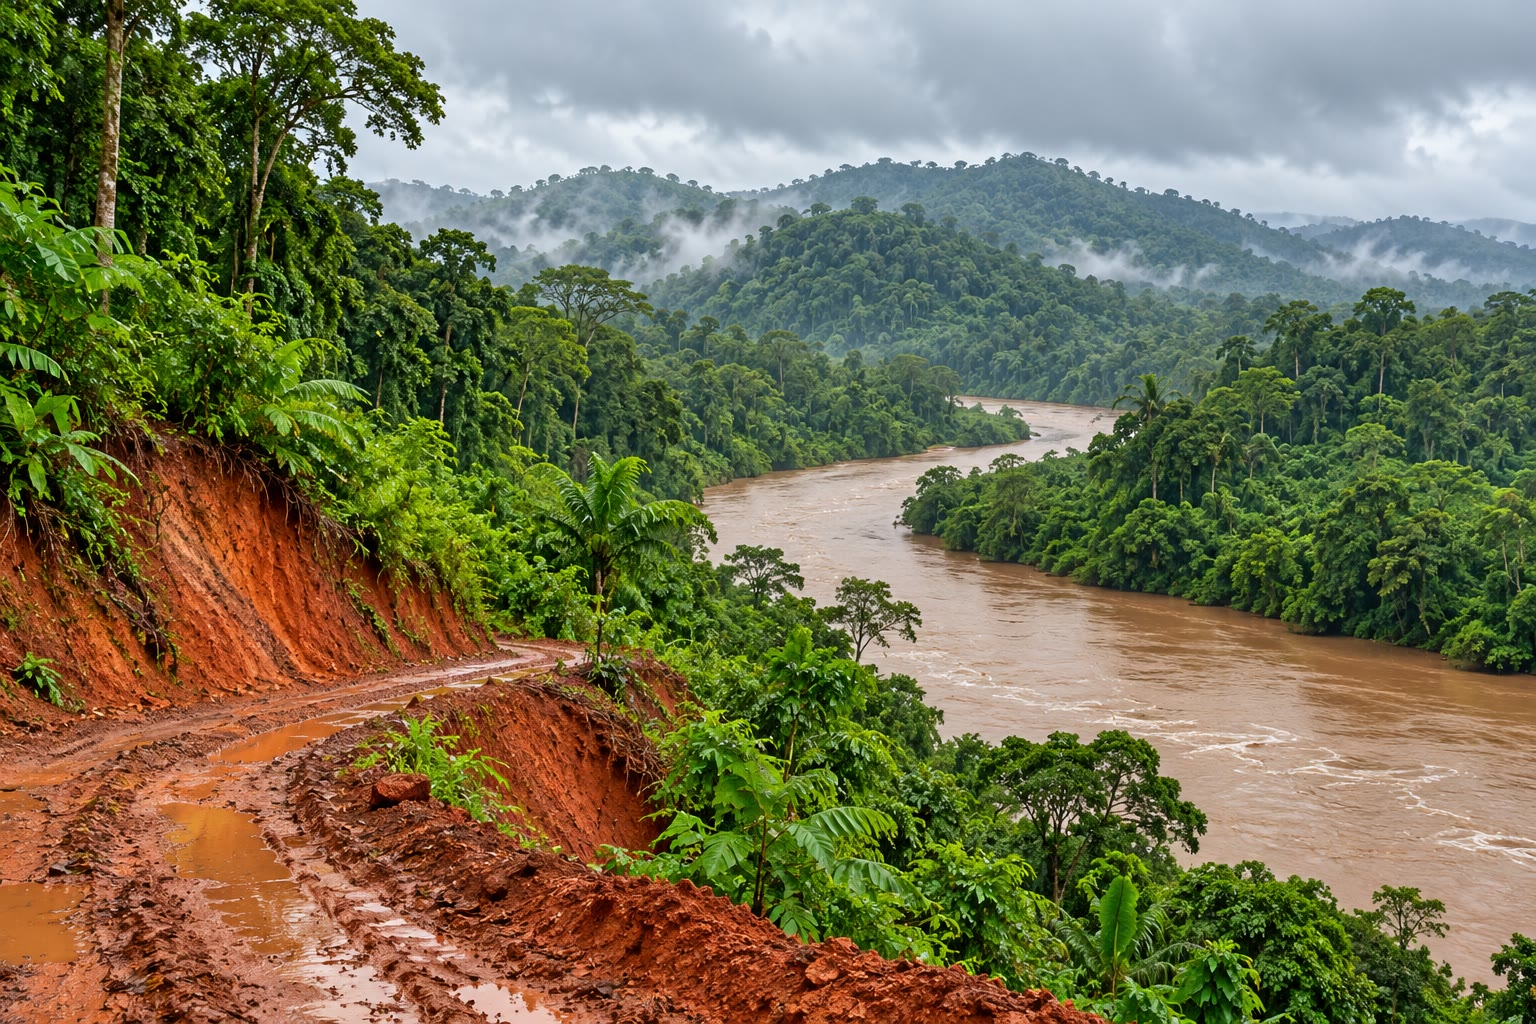
\includegraphics[width=0.66\linewidth]{images/book4/ai/b2-tropical-weathering.jpg}
\par\smallskip{\small Where the thermostat works hardest: a hot, wet lowland, where rain falls on
deeply weathered red soil and the river carries the products of weathering to the sea
(AI-generated illustration).}
\end{omfigure}

\section*{Exercises}\label{sec:b2:deep-time-climate:exercises}

Data for the exercises, unless stated otherwise: pre-industrial carbon in the atmosphere
\qty{591}{PgC} (\qty{278}{ppm}); $\qty{1}{Tmol}$ of carbon $= \qty{0.012011}{PgC}$; silicate
weathering $W_0 = \qty{0.138}{PgC.yr^{-1}}$; airborne share of an excess after the ocean and the
carbonates $f = 0.08$; weathering sensitivity $k_T = \qty{0.09}{K^{-1}}$; climate sensitivity $S =
\qty{3}{K}$; forcing of a doubling of carbon dioxide \qty{3.93}{W.m^{-2}}; $R =
\qty{8.314}{J.mol^{-1}.K^{-1}}$.
% ledger: ar6ch5:fig512, ipcc:erf-2xco2, derry24:fluxes, colbourn13:timescale, colbourn13:weathering, ipcc:ecs

\begin{exercise}[$\star$]\label{exo:b2:deep-time-climate:1}
Before the industrial era the ocean held \qty{900}{PgC} in its surface layer, \num{37100} in its
intermediate and deep water, 700 as dissolved organic carbon and 3 in its living organisms.
(a) How much carbon did the ocean hold, and how many times the atmosphere's? (b) Convert the
\qty{3.5e6}{Tmol} of the surface reservoirs to petagrams of carbon. (c) What share of it is in the
air?
\end{exercise}

\begin{exercise}[$\star$]\label{exo:b2:deep-time-climate:2}
Use the fluxes of the figure of the \omterm{def:b2:deep-time-climate:carbon-cycle}{long-term carbon cycle}, with metamorphic degassing taken as
\qty{3}{Tmol.yr^{-1}}. (a) Add up the inputs to the surface reservoirs and the outputs.
(b) What share of the inputs do volcanoes, rifts and \omterm{def:b2:metamorphic-facies:metamorphism}{metamorphism} supply? (c) Find the residence
time of carbon in the surface reservoirs, using the outputs.
\end{exercise}

\begin{exercise}[$\star$]\label{exo:b2:deep-time-climate:3}
(a) Write the weathering of forsterite, \ce{Mg2SiO4}, by carbon dioxide and water into magnesium
and bicarbonate ions and dissolved silica, \ce{SiO2}, and balance it. (b) The magnesium is later
deposited as carbonate. Write the net reaction. (c) What mass of forsterite must be weathered to
remove \qty{1}{PgC} for good? ($M(\ce{Mg2SiO4}) = \qty{140.7}{g.mol^{-1}}$.)
\end{exercise}

\begin{exercise}[$\star$]\label{exo:b2:deep-time-climate:4}
Put in order of age, with their dates, and say for each whether the Earth was in a greenhouse or
icehouse state: the Early Eocene Climatic Optimum; the Hirnantian glaciation; the onset of the
Antarctic ice sheet; the Turonian; the greatest ice extent of the late Palaeozoic; the major
advances of the northern ice sheets; the PETM.
\end{exercise}

\begin{exercise}[$\star\star$]\label{exo:b2:deep-time-climate:5}
(a) Check that an activation energy of \qty{63}{kJ.mol^{-1}} at \qty{288}{K} gives $k_T =
\qty{0.09}{K^{-1}}$. (b) Find $k_T$ for the field value \qty{74}{kJ.mol^{-1}}. (c) With each, find
the steady warming when the degassing rises by \qty{20}{\percent}. (d) Why does the climate
sensitivity not enter (c)?
\end{exercise}

\begin{exercise}[$\star\star$]\label{exo:b2:deep-time-climate:6}
Compare the exact Arrhenius factor $\exp[-(E_{\text a}/R)(1/T - 1/T_0)]$ with $e^{k_T(T -
T_0)}$, $k_T = E_{\text a}/(RT_0^2)$, for $E_{\text a} = \qty{63}{kJ.mol^{-1}}$ and $T_0 =
\qty{288}{K}$: (a) at $T = \qty{293}{K}$; (b) at $T = \qty{318}{K}$. (c) Show that the ratio of the
approximation to the exact factor is $\exp[E_{\text a}x^2/(RT_0^2(T_0 + x))]$, with $x = T - T_0$,
and find the warming at which it reaches 1.1.
\end{exercise}

\begin{exercise}[$\star\star$]\label{exo:b2:deep-time-climate:7}
The smoothed compilation gives \qty{1444}{ppm} of carbon dioxide at \qty{419.5}{Ma} and
\qty{276}{ppm} at the end of its record. (a) Find the forcing of that decline. (b) Compare it with
the \qty{9}{W.m^{-2}} of the brightening Sun. (c) Find the mean rate of decline in ppm per million
years, and compare it with the \qty{3.4}{ppm} of the fitted trend. Why may they differ?
\end{exercise}
% ledger: data:b4-foster2017, foster17:co2

\begin{exercise}[$\star\star$]\label{exo:b2:deep-time-climate:8}
(a) Spread \num{3000} and \qty{7000}{PgC} over 3 and over \qty{20}{kyr}: what range of release
rates follows? Compare with the 0.3 to \qty{1.5}{PgC.yr^{-1}} the IPCC quotes. (b) Human emissions
were about \qty{35}{Gt} of carbon dioxide in 2010. Convert to carbon and compare. (c) Carbon
dioxide rose from 900 to \qty{2000}{ppm}. Find the forcing and the equilibrium warming with $S =
\qty{3}{K}$, and compare with the \qty{5}{\celsius} of warming over the pre-PETM climate.
\end{exercise}
% ledger: ar6ch5:petm-release, usgs:volcanic-co2, ar6ch5:petm

\begin{exercise}[$\star\star$]\label{exo:b2:deep-time-climate:9}
The rise of a mountain belt multiplies the Earth's weatherability $W_0$ by 1.2, at a constant
degassing. (a) Find the new steady temperature change. (b) Find the new steady carbon dioxide, from
\qty{278}{ppm}. (c) Does the rate of silicate weathering, at the new steady state, differ from the
old one? Explain.
\end{exercise}

\begin{exercise}[$\star\star\star$]\label{exo:b2:deep-time-climate:10}
(a) Find the thermostat's e-folding time with the run-off factor, $k = 0.09 + 0.65\times0.045$.
(b) Over millions of years the ice sheets and the vegetation respond too; with an Earth system
sensitivity of \qty{8}{K} per doubling instead of $S$, find $\tau$ with $k_T$. (c) Which way do the
two changes push the thermostat, and which uncertainty, $E_{\text a}$ or $S$, matters more?
\end{exercise}

\begin{exercise}[$\star\star\star$]\label{exo:b2:deep-time-climate:11}
A release of \qty{5000}{PgC} (after the ocean and the carbonates). (a) Find the carbon dioxide of
the air, in ppm, and the warming. (b) Find the initial net removal rate $W - W_0$, and the time the
pulse would take to vanish at that rate. (c) Find the linearised time to remove \qty{90}{\percent}
of the excess. (d) The model, integrated without linearising, takes \qty{340}{kyr}. Why longer?
\end{exercise}

\begin{exercise}[$\star\star\star$]\label{exo:b2:deep-time-climate:12}
(a) Linearise the model about a steady state where the degassing is $V$ and $C = C^*$, and show that
the e-folding time is $\tau' = A_0 (C^*/C_0)\ln 2/(f k S V)$. (b) Evaluate it for the steady state
of a \qty{20}{\percent} rise in degassing. (c) Is the thermostat faster or slower in a world rich in
carbon dioxide, and why?
\end{exercise}

\begin{problem}[{Weekend problem --- How long does the thermostat take?}]\label{pb:b2:deep-time-climate:1}
This problem builds the thermostat's time constant from measured fluxes. Use the data of the
exercises; degassing at ridges, ocean islands, arcs and rifts \num{1.3}, \num{1.3}, 4.5 and
\qty{4.2}{Tmol.yr^{-1}}; silicate weathering 11 to \qty{12}{Tmol.yr^{-1}}; activation energy
\qty{63}{kJ.mol^{-1}} at $T_0 = \qty{288}{K}$; mass of the atmosphere \qty{5.1e18}{kg}, mean molar
mass of air \qty{28.97}{g.mol^{-1}}. Round to three significant figures.

\noindent\textbf{Part I --- Balance.}
\begin{enumerate}
  \item Add up the volcanic and rift degassing, in \unit{Tmol.yr^{-1}} and in \unit{PgC.yr^{-1}}.
  \item Take $W_0$ in the middle of its range; convert it to \unit{PgC.yr^{-1}}.
  \item Compare the two. What does the comparison suggest about the \omterm{def:b2:deep-time-climate:carbon-cycle}{long-term carbon cycle}?
  \item How many moles of air does the atmosphere hold? How many moles of carbon are \qty{591}{PgC},
        and what mixing ratio is that?
  \item With no weathering at all, how long would the degassing of question 1 take to add
        \qty{591}{PgC} to the surface reservoirs?
  \item If a fraction $f = 0.08$ of that stayed in the air, by what factor would the air's carbon
        dioxide rise?
\end{enumerate}

\noindent\textbf{Part II --- Linearising.}
\begin{enumerate}[resume]
  \item Find $k_T$ from the activation energy, and check that it rounds to the
        \qty{0.09}{K^{-1}} used below.
  \item By what factor does the weathering grow for a warming of \qty{1}{K}?
  \item Write the warming $\Delta T$ for an excess $M$, and its derivative at $M = 0$, in
        \unit{K.PgC^{-1}}.
  \item Find the derivative of $W$ with respect to $M$ at $M = 0$, in \unit{yr^{-1}}.
  \item Show that its inverse is the time constant $\tau$ of
        \cref{prop:b2:deep-time-climate:thermostat}.
  \item Which of $f$, $k$, $S$ and $W_0$ make the thermostat faster when they increase?
\end{enumerate}

\noindent\textbf{Part III --- The time constant.}
\begin{enumerate}[resume]
  \item Evaluate $\tau$.
  \item Evaluate it with the run-off factor, $k = \qty{0.119}{K^{-1}}$.
  \item Evaluate it with $k_T$ and an activation energy of \qty{74}{kJ.mol^{-1}}.
  \item Compare these values with the \qty{200}{kyr} to \qty{1}{Myr} of models with an explicit ocean.
  \item How many e-folding times fit into the \qty{50}{Myr} of the Cenozoic decline of carbon
        dioxide? What does that say about the state of the carbon cycle during the decline?
  \item At \qty{16}{ppm} per million years, how much does carbon dioxide change in one $\tau$?
\end{enumerate}

\noindent\textbf{Part IV --- A PETM-sized release.}
\begin{enumerate}[resume]
  \item \qty{5000}{PgC} is released; how much stays in the air after the ocean and the carbonates
        have acted, and what is the carbon dioxide in ppm?
  \item Find the warming at that moment.
  \item By how much does the weathering rate rise, in \unit{PgC.yr^{-1}} and in per cent?
  \item With the linearised law, how long until \qty{90}{\percent} of the excess is gone?
  \item The PETM's carbonate recovered over about \qty{100}{kyr}. Give two reasons why the real
        Earth may have been faster than this model.
  \item To sum up: what is the e-folding time of the \omterm{def:b2:deep-time-climate:thermostat}{silicate-weathering thermostat} in this model?
\end{enumerate}
\end{problem}
% ledger: derry24:fluxes, colbourn13:weathering, colbourn13:timescale, ar6ch5:fig512, ar6ch5:petm, ar6ch5:cenozoic-co2, ipcc:ecs, earth:Matm, earth:Mmol
